\chapter{硬件设计}

\section{信号放大电路}

在光电探测系统中,探测器输出的电信号非常微弱,一般为毫伏级。为记录每一次打靶的结果,信号放大与处理电路是打靶系统中不可或缺的。在探测器上直接进行信号处理十分困
难,一种常用的解决办法是在探测器后接前置放大器,用来放大探测器的输出信号,然后成
功地传输到信号处理系统的有关电路部分。前置放大器的设计要求是低噪声,高增益,低输
出阻抗,大的动态范围,和较好的抗噪声能力。

在激光打靶系统中,对光电池产生的脉冲信号的具体大小值要求不高,只需检测出有效的脉
冲信号,因此可选用集成运放来组成运算放大电路。

通过测试,得到光电探测器对的激光脉冲的响应幅度典型值约为$\qty5\mV$,若激光击中
在两块或多块探测器边界处,则任何一块光电探测器的响应幅度会减少,因此所检测的脉冲
幅度范围大约是$\num3\sim\qty5\mV$.为使每块光电探测器均能检测出信号,使之达到
TTL 电平要求,实现信号检测,必须对信号放大约 1000 倍。单级运放难以达到这么高的
放大倍数,因此采用二级运放进行放大,第一级为前置放大器。为减少前级放大器的偏移对
后级放大器的影响,设计其放大倍数$A_1=100$;从而次级放大器的放大倍数$A_2=10$。

\subsection{集成运算放大器(LM324)}

集成运算放大器是实现高增益放大功能的一种集成器件\cite{cn9},早期主要用来实现对模拟量进行
数学运算的功能,目前随着器件性能的改进,它已成为通用的增益器件,应用范围非常广泛。

从电特性来看,集成运放接近理想的电压放大器件,它不仅有很大的输入电阻和很小的输出
电阻,而且还有很高的电压增益,此外,静态工作时,它的输入和输出电位均为零,这样,
在与其它集成运放连接时,就不需要考虑它们之间的电平配置问题。

LM324 是四通道的低功耗运算放大器,它的内部包含四组形式完全相同的运算放大器,除电
源共用外,四组运放相互独立,其性能参数有以下几个方面:

\begin{enumerate}
  \item 单电源工作方式,工作电平$\qty3\V\sim\qty{30}\V$
  \item 低消耗电流:约$\qty{0.8}\mA$
  \item 低输入偏移:输入电压偏移:$\qty3\mV$(Typ);输入电流偏移:$\qty2\nA$(Typ)
  \item 开环增益:$\qty{100}\V/\unit\mV=\qty{100}\dB$(Typ)
  \item 宽响应频带
\end{enumerate}

\newpage
\begin{figure}[htbp]
  \centering
  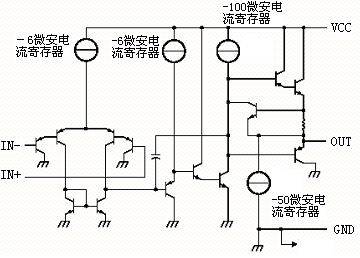
\includegraphics[width = .595\linewidth]{image-0162}
  \caption{LM324内部结构}
  \label{4-1}
\end{figure}

\subsection{放大电路图}

\begin{figure}[htbp]
  \centering
  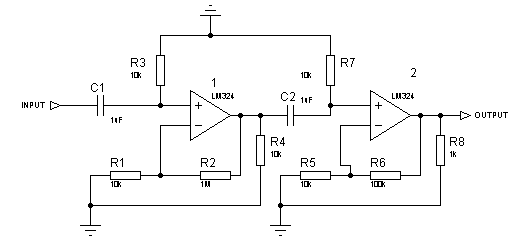
\includegraphics[width = .93\linewidth]{image-0163}
  \caption{运算放大器电路图}
  \label{4-2}
\end{figure}

放大器电路如\cref{4-2} 所示。它由两级结构相同的同相放大器组成,集成放大器选用
LM324(\cref{4-1})。信号经隔直流电容C1从第一级放大器的正端
``\ensuremath+''输入,经过放大后输出,再经过级间耦合电容C2输入第二级放大器
的正端。前级的放大倍数$A_1=R_2/R_1=100$,后级的放大倍数$A_2=R_6/R_5=10$,
$R_3$和$R_7$为输入匹配电阻。

\subsection{电路原理}

\begin{enumerate}
  \item 同相放大器\cite{cn10}(\cref{4-3})
  
  集成运放是一种十分理想的增益器件,性能好,使用方便。该电路采用 2 级放大器级
  联,每级的放大器均采用同相放大。

  由集成运放构成的同相放大器,其特点是输入信号加在同相输入端,而反馈信号加在反相端。根据理想化条件,由于$v_+=v_s$,因而$v_-\approx v_s$。更具$i\to0$(虚断),$v_-$又是$v_o$在$R_1$上的分压值,即:
  \begin{equation}
    v_-=v_o\frac{R_1}{R_1+R_f}
  \end{equation}
  因而,放大器的增益:
  \begin{equation}
    A_{Vf}=\frac{v_o}{v_s}=\frac{R_1+R_f}{R_1}=1+\frac{R_f}{R_1}
  \end{equation}
  $\because A_{Vf}>0$,所以$v_o$与$v_s$同相。
  
  \begin{figure}[htbp]
    \centering
    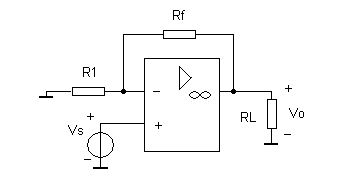
\includegraphics[width = .54\linewidth]{image-0236}
    \caption{同相放大器}
    \label{4-3}
  \end{figure}
  \item 外围电路
  
  光电传感器对外部光线也有响应,因此必须滤除这种干扰。由于背景光线是持续信号,其
  响应主要是直流量,在第一级放大器输入端的前面设计接入一个$\qty1\uF$电容C1起到
  隔离直流作用,能起到很好的效果。第二级的$\qty1\uF$电容C2用于两级放大器的耦合。

  第一级放大器输入端和地之间接 R3;第二级放大器输入端和地之间接 R7。使得:
  \begin{equation}
    \begin{cases}
      R_3\approx R_1//R_2\\
      R_7\approx R_5//R_6
    \end{cases}
  \end{equation}
  这样,运放的正、负输入端对地的等效电阻相等,从而降低运放的电压偏移。
\end{enumerate}

\subsection{电路参数}

\begin{enumerate}
  \item \makebox[9em][l]{输入脉冲幅度:} $U_i\approx\num3\sim\qty5\mV$
  \item \makebox[9em][l]{输入电阻:} $R_i\approx\qty{10}\kohm$
  \item \makebox[9em][l]{输出电阻:} $R_o\approx\qty1\kohm$
  \item \makebox[9em][l]{放大倍数:} $A=A_1\cdot A_2\approx10\times100=1000$
  \item \makebox[9em][l]{放大器级数:} 两级,前级$A_1\approx100$;后级$A_2\approx10$
  \item \makebox[9em][l]{耦合方法:} 电容耦合
\end{enumerate}

\clearpage
\vspace*{-1.5em}
\section[整形电路]{整形电路\cite{cn11}}

光电池的输出脉冲并不是规则的矩形脉冲信号,而是类似升余弦信号。再经放大后也会产生
失真,因此必须对信号进行整形。采用常用的 CD4093 施密特触发器便可实现整形功能,改
善脉冲波形,确保后续编码器的正常编码。

施密特触发器不仅可以进行波形整形,它的迟滞特性还可以有效地克服噪声和干扰的影响,只要噪声和干扰的大小处在迟滞宽度内,就不会有错误的输出。施密特触发器属于电平触
发,对于缓慢变化的信号仍然适用,当输入信号达到阈值电压时,电路状态发生转换,通过
电路内部的正反馈过程使得输出电压的波形的边沿变得很陡峭。利用施密特触发器可以实现
有效脉冲的识别见\cref{4-5}。

\begin{figure}[htbp]
  \centering
  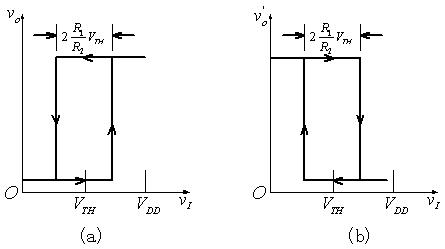
\includegraphics[width = .65\linewidth]{image-0284}
  \caption{施密特触发器的电压传输特性\quad (a) 同相输出;(b) 反相输出}
  \label{4-4}
\end{figure}

\begin{figure}[htbp]
  \centering
  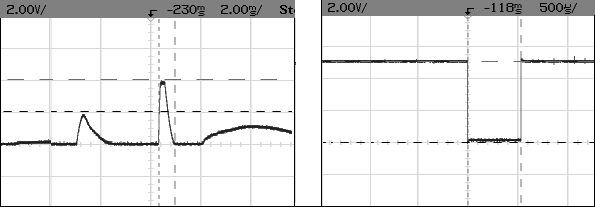
\includegraphics[width = .95\linewidth]{image-0285}
  \caption{利用施密特触发器实现有效脉冲的识别}
  \label{4-5}
\end{figure}

\section[编码电路]{编码电路\cite{cn11}}

对于 38 路信号通道,必须对其进行编码以便于信号识别和传输。38 路信号按照设计方案
编码为 1--38 号,脱靶无信号记为 0 号。对多个探测器同时接收到信号的情况,对应于
探测器的码号就是取码号大的探测器为有效,采用优先编码器便可实现编码的优先选择。

商用的单个优先编码器的编码输入最多只有 8 路,要构成更多路的优先编码
器,可以采用 6 片 8-3 优先编码器进行扩展为 40-6 优先编码器。

\subsection{编码电路图}

\begin{figure}[htbp]
  \centering
  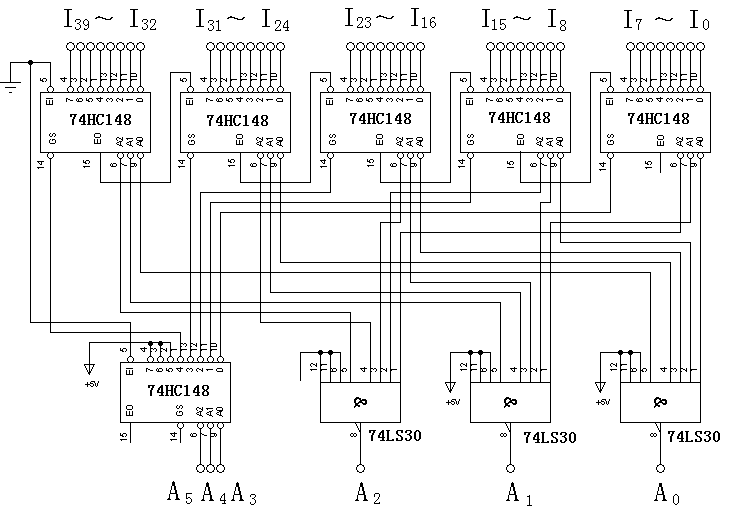
\includegraphics[width = .93\linewidth]{image-0289}
  \caption{40-6 优先编码器电路图}
  \label{4-6}
\end{figure}

\subsection{电路原理}

\begin{enumerate}
  \item 优先编码器(74HC148)
  
  8-3 线优先编码器的功能表如\cref{4-7}。待编码的 8 条输入线 采用 8 中取 1 
  码,逻辑 0 有效,编码后的输出 用反码表示。可以看出,编码器是以输入为 0 的最高
  优先编码的,而低位若同时输入 0,则是无意义的。此外,电路还设有选通输入,即使能
  端 EI,它也是逻辑 0 有效;输出还设有允许输出端 Eo 及允许扩展端 Gs,利用它们
  可判断出 是否有效,以及是否允许扩展编码。根据真值表,写出编码器的逻辑表达式如下:
  \begin{equation}
    \begin{aligned}
      \overline{A_2}&=\overline{EI}\cdot I_7+\overline{EI}\cdot I_7\cdot I_6\cdot\overline{I_5}+\overline{EI}\cdot I_7\cdot I_6\cdot I_5\cdot\overline{I_4}\\
      &=\overline{EI}(\overline{I_7}+I_7\overline{I_6}+I_7I_6I_5\overline{I_4})=\overline{EI}(\overline{I_7}+\overline{I_6}+\overline{I_5}+\overline{I_4})
    \end{aligned}
  \end{equation}
  故:
  \begin{equation}
    A_2=\overline{\overline{EI}(\overline{I_7}+\overline{I_6}+\overline{I_5}+\overline{I_4})}
  \end{equation}
  同理:
  \begin{gather}
    A_1=\overline{\overline{EI}(\overline{I_7}+\overline{I_6}+I_5I_4\overline{I_3}+I_5I_4I_2)}\\
    A_0=\overline{\overline{EI}(\overline{I_7}+I_6\overline{I_5}+I_6I_4\overline{I_3}+I_6I_4I_2\overline{I_1})}
  \end{gather}
  而允许输出为:
  \begin{equation}
    E_OE_0=\overline{\overline{EI}\cdot I_7I_6I_5I_4I_3I_2I_1I_0}
  \end{equation}
  允许扩展端是:
  \begin{equation}
    Gs=EI+\overline{EI}\cdot I_7\;I_6\;I_5\;I_4\;I_3\;I_2\;I_1\;I_0=\overline{\overline{EI}\cdot E_O}
  \end{equation}

  \begin{table}[htbp]
    \centering\scriptsize
    \renewcommand\arraystretch{1.12}
    \begin{tabular}{|>{\centering\arraybackslash\sffamily}p{.04\linewidth}|*{8}{>{\centering\arraybackslash\sffamily}p{.04\linewidth}}|*{3}{>{\centering\arraybackslash\sffamily}p{.04\linewidth}}|*{2}{>{\centering\arraybackslash\sffamily}p{.04\linewidth}}|}
      \hline
      \multicolumn{9}{|>{\sffamily\bfseries}c|}{INPUTS} & \multicolumn{5}{>{\sffamily\bfseries}c|}{OUTPUTS}\\
      \hline
      EI & 0 & 1 & 2 & 3 & 4 & 5 & 6 & 7 & A2 & A1 & A0 & GS & EO\\
      \hline
      H & X & X & X & X & X & X & X & X & H & H & H & H & H\\
      L & H & H & H & H & H & H & H & H & H & H & H & H & L\\
      L & X & X & X & X & X & X & X & L & L & L & L & L & H\\
      L & X & X & X & X & X & X & L & H & L & L & H & L & H\\
      L & X & X & X & X & X & L & H & H & L & H & L & L & H\\
      L & X & X & X & X & L & H & H & H & L & H & H & L & H\\
      L & X & X & X & L & H & H & H & H & X & L & L & L & H\\
      L & X & X & L & H & H & H & H & H & X & L & H & L & H\\
      L & X & L & H & H & H & H & H & H & X & H & L & L & H\\
      L & L & H & H & H & H & H & H & H & X & H & H & L & H\\
      \hline
    \end{tabular}
    \caption{8-3 线优先编码器真值表(74HC148)}
    \label{4-7}
  \end{table}
  \item 8-3 线优先编码器扩展为 40-6 线优先编码器(\cref{4-6})
  
  5 片 74HC148 并排用作输入,其输入从低位片到高位片排列为
  $I_0\sim I_{39}$ 。每一个高位片的输出允许端 Eo 接其相对低位片的使能端 EI。这样,当总使能$\text{EI}=0$时,允许电路进行编码工作,若高位片的诸输入中有一
  个为$0$时,该片的 $\text{Eo}=1$,$\text{Gs}=0$,这样就禁止了低位片的编
  码,以此类推,5 片 74HC148 的输入端编码便具有了优先性。

  5 片 74HC148 的允许扩展端 Gs 按低位片至高位片的顺序分别接到第六片74HC148
  的$I_0$、$I_1$、$I_2$、$I_3$、$I_4$输入端,而$I_5$、$I_6$、$I_7$端则接
  高电平(表示无输入)。这样第六片 74HC148 的三位输出便表示整个 40-6 线优先编
  码器的高三位$A_5$、$A_4$、$A_3$。而 40-6 线优先编码器的低三位输出$A_2$、$A_1$、$A_0$与前 5 片 74HC148 的输出端一致。

  由于 74HC148 的输出端不是三态门,不能直接连接在一起。而把 5 片 74HC148的同
  名输出端接到 74LS30(8 输入的与非门)取与非便可以解决这个问题。同时输出取反,
  输出为逻辑 1 有效。为使高三位输出与低三位输出一致,用 CD4049反相器对高三位取
  反。
  
  40-6 线优先编码器的六个输出均为逻辑 1 有效,可以接到后续的 2051 单片机进行串
  行传输。
\end{enumerate}

\section{串行传送}

为实现将编码器输出的 6 位并行信号串行传送,同时实现数据发送和打靶射击的同步性。采
用 89C2051 单片机便可实现要求。

\subsection{单片机及外围电路图}

\begin{figure}[htbp]
  \centering
  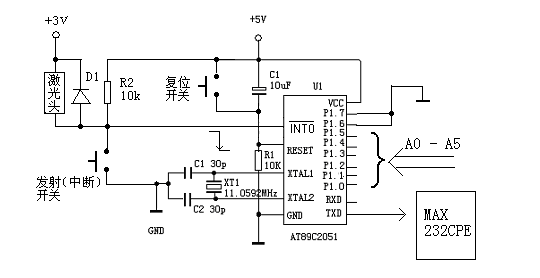
\includegraphics[width = .9\linewidth]{image-0419}
  \caption{2051 单片机及其外围电路图}\label{4-8}
\end{figure}

\subsection{电路原理}

\begin{enumerate}
  \item 编码器的输出通过 2051 P1 口的低 6 位(高 2 位接地为逻辑 0)输入。
  \item 选用 $\qty{11.0592}\MHz$ 的晶振构成单片机的时钟,这样在串口工作方式 1 下可得到准确的 $\qty{9600}{bps}$ 的串行波特率,方便计算机的接收。
  \item 单片机接有复位开关按钮。
  \item 实现打靶和信号采集传送的同步化。
\end{enumerate}

由于采用单片机的外部中断 0($\overline{INTO}$)作为数据串行传送的使能端,且
$\overline{INTO}$设为下降的跳变沿有效。使能开关(激光枪的开关)一端接地,另一
端接$\overline{INTO}$,又经上拉电阻接到电源,这样当开关按下时,便有下降沿的跳变信号输入$\overline{INTO}$,产生中断。

同时,开关又要同步控制激光枪的发射。因此开关又接激光头的负端,从而控制激光头负端
的接地,只有当开关按下时,激光头两端才有工作电压。

这样,同一个开关既控制单片机的中断,又同时控制激光枪的发射,从而达到打靶和信号采
集传送这两个“动作”的同步化。

\subsection{AT89C2051 单片机\cite{cn12}}

AT89C2051 单片机是 AT89C51 的简化型号,其指令系统和内部 RAM 均与 AT89C51相
同。不同的是它的内部 ROM 为 2k,而 89C51 为 4k,而且 2051 比 89C51 少了 P0
和 P2 输入/输出口以及外部 ROM、RAM 的扩展端,因此在引脚上 2051 只有 20 个脚。
AT89C2051 单片机主要适用于较为简单的微控制系统。在本系统中,用到 AT89C2051的 
6 个外部 I/O 口,一个外部中断和串行输出口。

\newpage
\begin{figure}[htbp]
  \centering
  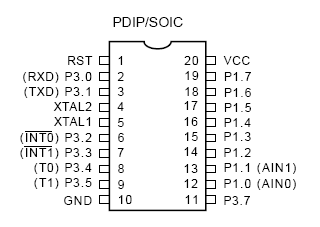
\includegraphics[width = .53\linewidth]{image-0439}
  \caption{2051 信号引脚图}
  \label{4-9}
\end{figure}

\section{电平转换}

在不同的数字系统中,其电平标准是不同的。该系统中就包括了 TTL 电平标准和 RS-232 
电平标准,要实现两个标准的正常通信,必须进行电平转换。该系统采用使用简单的 
MAX232CPE 芯片。

一片MAX232CPE芯片可完成2路TTL/CMOS~RS-23 的电平转换和2路RS-232~TTL/CMOS
的电平转换。实际电路中只有一路单片机的 TXD 串口输出,不进行RXD串口输入。因此,选
用引脚 11 接 2051 TXD 串口输出;而对应的 14 脚则接到计算机的串口输入端。

\begin{figure}[htbp]
  \centering
  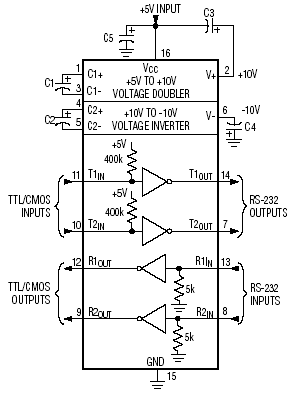
\includegraphics[width = .52\linewidth]{image-0440}
  \caption{MAX232CPE 芯片内部结构}
  \label{4-10}
\end{figure}